Every robotic system has some set of parameters---scale factors, sensor
locations, link lengths, etc.---that are needed for state estimation, planning,
and control. Despite best efforts during construction, some parameters will
change over the lifetime of a robot due to normal wear and tear. In the best
case, incorrect parameter values degrade performance. In the worst case, they
cause critical safety issues.

We are interested in developing automated systems that are capable of robust
long-term deployment in the hands of non-experts, so the identification and
update of these parameter values is highly important.

As an example, consider a camera-based collision avoidance system intended for
deployment in a consumer automobile. For the vehicle to be able to avoid
collisions, the pose of each camera with respect to the vehicle coordinate
system must be known precisely so that obstacle positions can be transformed
from camera coordinates into vehicle coordinates. However, a consumer vehicle
will have no access to special calibration hardware or expert data analysis.
In such a scenario, the vehicle must be capable of self-supervised
recalibration. This problem is inherently difficult for a number of reasons that
we will briefly discuss here.

{\bf 1) Parameters change over time}---although the vehicle may be factory
calibrated, the transformations can change slowly over time due to vibration,
thermal expansion, loose parts, or any number of other common problems that
follow from normal usage.

{\bf 2) Parameters must be inferred from the data}---as the cameras may be
installed in different places on the vehicle, their pose cannot be measured
directly. Instead, the transformations must be inferred from the data produced
by the full system. However, this is only possible if the motion of the vehicle
renders the parameters {\em observable}\footnote{Informally, observability
means that the parameters can be inferred from some local batch of measurement
data~\cite{jazwinski70stochastic}}.

{\bf 3) Normal operation may result in unobservable directions in parameter
space}---unfortunately, for this and many other practical problems normal
operation may not render all directions in parameters space observable. In this
example, when two cameras do not share an overlapping field of view, planar
motion renders the calibration problem
degenerate\footnote{See~\cite{lebraly10calibration} for a handy table of
degenerate cases or \cite{kim06absolute} for a more theoretical analysis.}; the
transformation between cameras only becomes observable under general 3D motion.

{\bf 4) Unobservable directions in parameter space may appear observable in the
presence of noise}---even if our hypothetical car is piloted only on a plane (a
degenerate case), noise in the measurements can make unobservable parameters
appear observable. We call these parameters {\em numerically unobservable} to
mirror the related concept of numerically rank-deficient matrices.

\begin{figure}[t]
\centering
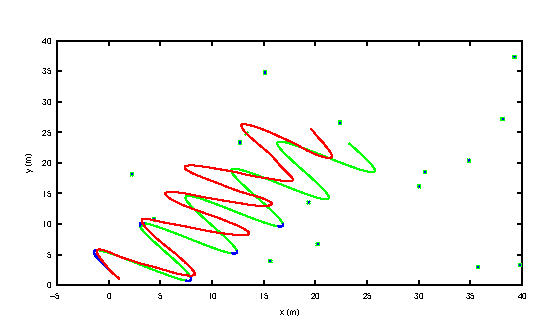
\includegraphics[width=\columnwidth]{fig/sin-path-result.eps}
\caption{Exemplary output of our calibration algorithm (best viewed in
color). The ground truth trajectory and landmark positions are shown in green
and their respective estimates in blue. While dealing with degenerate cases, our
method only selects batches of data that provide enough information to the
estimator.}
\label{fig:calib_demo}
\end{figure}

Existing algorithms for self calibration generally handle issues (1) and (2).
Issue (3) is dealt with by designing experiments that guarantee all parameters
become observable. To the best of our knowledge, no published self-calibration
algorithm is able to cope with issue (4). Therefore, unless we plan to require
all vehicle owners to outfit their parking places with calibration patterns or
regularly drive off-road, new advances for online system calibration are
required.

In this paper, we propose an algorithm to deal with {\em all} of these
difficulties. Our approach exploits the algebraic links between the Gauss-Newton
algorithm, the Fisher Information Matrix, and non-linear observability analysis
to automatically detect directions in parameter space that are numerically
unobservable and avoid updating our parameters in these directions; at any given
time, directions in the parameter space that are observable will be updated
based on the latest information, while unobservable directions will remain at
their initial guess. Novel sets of measurements are detected using a mutual
information test, and added to a working set that is used to estimate the
parameters. The result is an algorithm that listens to an incoming stream of
data, automatically accumulating a batch of data that may be used to calibrate a
full robot system. The only requirements are that (i) the parameters are
theoretically observable given some ideal set of data, (ii) it is possible to
implement a batch Gauss-Newton estimator for the system state and calibration
parameters based on a set of measurements, and (iii) we have some reasonable
initial guess for the calibration parameters (e.g. from factory calibration).
Fig.~\ref{fig:calib_demo} shows a typical calibration run of our algorithm.

The remainder of the paper is structured as follows. Section~\ref{sec:rel}
will give a brief overview over related approaches. Section~\ref{sec:model} is
dedicated to the mathematical grounding of our method.
Section~\ref{sec:exp} demonstrates the validity of our approach through
extensive experiments and evaluation. Section~\ref{sec:conc} will conclude the
paper.
